\bookchapter{บทที่ 42: ภาพรวมโมเดลใหญ่และการใช้ API จริง}

\chapterintro{หลายบทที่ผ่านมาพูดเรื่อง “ทำงานร่วมกับ AI อย่างไร” บทนี้จะแก้ปัญหาที่พื้นฐานกว่านั้น: “ใช้ AI ตัวไหน? ใช้อย่างไร?” ภูมิทัศน์โมเดลใหญ่เมื่อเดือนสิงหาคม 2026 รุ่มรวยมาก — ฝั่งสากลมีศึกสามเสือ GPT, Claude, Gemini ส่วนฝั่งจีนมี DeepSeek, Qwen, GLM, Kimi, Doubao เบ่งบานกันทั้งวงการ แต่ละโมเดลมีอุปนิสัยและความถนัดของตัวเอง: เลือกถูกตัวก็ได้ผลคุ้มค่า เลือกผิดก็เหนื่อยเปล่าเปลืองเงิน บทนี้ไม่เพียงพาคุณไปรู้จักโมเดลเหล่านี้ แต่ยังสอนวิธีต่อพวกมันเข้ากับแอปของคุณผ่าน API และวิธีเลือก Token Plan (แพ็กเกจโควตาการใช้งาน) ให้เหมาะกับความต้องการของตัวเอง}

\booksection{โมเดลใหญ่หลักสากล: สามเสือคุมเกม}

ตลาดโมเดลใหญ่สากลในเดือนสิงหาคม 2026 ก่อรูปเป็นแบบสามเสือแย่งชิง: OpenAI (ตระกูล GPT), Anthropic (ตระกูล Claude), Google (ตระกูล Gemini) แต่ละเจ้ามีเอกลักษณ์ชัดเจนของตัวเอง — ไปรู้จักกันทีละตัว

\booksubsection{ตระกูล OpenAI GPT-5.6: นักสู้รอบด้านที่สมดุลทุกด้าน}

OpenAI คือผู้เปิดม่านคลื่นโมเดลใหญ่ และตระกูล GPT ยังเป็นโมเดลที่ใช้แพร่หลายที่สุดในโลกถึงวันนี้ ตระกูล GPT-5.6 ที่เปิดตัวเมื่อกรกฎาคม 2026 ใช้กลยุทธ์วางตำแหน่งสามระดับ: รุ่นเรือธง GPT-5.6 Sol สำหรับงาน reasoning ระดับสูง รุ่นสมดุล GPT-5.6 Terra สำหรับพัฒนางานประจำวัน และรุ่นเบา GPT-5.6 Luna สำหรับสถานการณ์ที่ต้องรองรับการเรียกใช้พร้อมกันจำนวนมากแบบต้นทุนต่ำ โมเดลทั้งสามใช้ context window ร่วมกันที่ 1.05 ล้าน Token รองรับทั้ง input รูปภาพ การเรียกใช้ฟังก์ชัน และ structured output

\begin{center}
\begin{tabularx}{\linewidth}{|X|X|X|X|X|}
\hline
\textbf{รุ่น} & \textbf{ระดับ} & \textbf{Input (/ล้าน Token)} & \textbf{Output (/ล้าน Token)} & \textbf{Context Window} \tabularnewline
\hline
GPT-5.6 Sol & เรือธง (reasoning) & US\$5.00 (ราว 36 หยวน) & US\$30.00 (ราว 217 หยวน) & 1.05 ล้าน Token \tabularnewline
GPT-5.6 Terra & สมดุล (งานประจำวัน) & US\$2.50 (ราว 18 หยวน) & US\$15.00 (ราว 109 หยวน) & 1.05 ล้าน Token \tabularnewline
GPT-5.6 Luna & เบา (ต้นทุนต่ำ) & US\$1.00 (ราว 7 หยวน) & US\$6.00 (ราว 44 หยวน) & 1.05 ล้าน Token \tabularnewline
\hline
\end{tabularx}
\end{center}

\begin{center}\small\color{gray}ราคาตระกูล OpenAI GPT-5.6 (สิงหาคม 2026)\end{center}

จุดแข็งหลักของตระกูล GPT อยู่ที่ “สมดุล” — reasoning, เขียนโค้ด, งานเขียน, มัลติโมดัล ไม่มีด้านไหนถ่อยชัดเจน บวกกับระบบนิเวศปลั๊กอินและชุมชนนักพัฒนามหาศาลของ OpenAI เอกสารรองรับและ toolchain จึงครบสมบูรณ์ที่สุด สำหรับสถานการณ์ “ไม่รู้จะเลือกอะไร” GPT คือคำตอบมาตรฐานแบบ “หลับตาเลือกก็ไม่ผิด” แต่จุดอ่อนของมันคือ: การเข้าถึงจากจีนต้องใช้เครือข่ายพิเศษ การสื่อสารภาษาจีนบางครั้งมี “กลิ่นคำแปล” และราคา API อยู่ระดับกลางถึงสูง

\textbf{ข่าวดี}\par

OpenAI ประกาศเมื่อสิงหาคม 2026 ว่าอัปเกรดโมเดลเริ่มต้นของผู้ใช้ฟรีเป็น GPT-5.6 Luna พร้อมเปิดแชทข้อความแบบไม่จำกัดปริมาณ นั่นแปลว่าคุณทดลองความสามารถพื้นฐานของ GPT ได้โดยไม่เสียค่าใช้จ่าย เสียเงินก็ต่อเมื่อต้องการ reasoning ที่แรงขึ้นหรือเรียกใช้ผ่าน API

\booksubsection{ตระกูล Anthropic Claude: เพดานสูงสุดด้านการเขียนโค้ดและความแม่นยำ}

ถ้า GPT คือนักกีฬาสารพัดสาย Claude ก็คือ “เพดาน” ของวงการเขียนโค้ด ตระกูล Claude ของ Anthropic นำโดด ๆ มายาวนานบน SWE-bench (benchmark ด้านวิศวกรรมซอฟต์แวร์) คุณภาพการสร้างโค้ดและความสามารถพาโปรเจกต์ระดับวิศวกรรมให้ลงตัวจริงติดอันดับหนึ่งของวงการ ที่หายากยิ่งกว่าคือ อัตรา hallucination (ความน่าจะเป็นที่จะสร้างข้อมูลเท็จ) ของ Claude ต่ำที่สุดในวงการ แค่ราว 1\% — ทำให้เหมาะเป็นพิเศษกับงานที่ต้องแม่นยำสูงอย่างวิชาการหรือกฎหมาย

อีกไม้ตายหนึ่งของ Claude คือบริบทยาวระดับสุด: รองรับ context window 1 ล้าน Token อ่าน “จบในรอบเดียว” ทั้งสัญญาหลายร้อยหน้าหรือโค้ดทั้งโปรเจกต์โดยไม่ตกหล่นรายละเอียด ความสามารถนี้แทบไม่มีตัวแทนในสถานการณ์อย่าง refactor โค้ดหรือวิเคราะห์เอกสารยาว Claude Code ในฐานะเครื่องมือเขียนโค้ด AI บนเทอร์มินัลมีรายได้เฉลี่ยต่อปีแตะ 2.5 พันล้านดอลลาร์สหรัฐแล้วตั้งแต่กลางปี 2026 — นั่นคือหลักฐานที่ชัดที่สุดว่าฝีมือเขียนโค้ดของ Claude ได้รับการยอมรับมากที่สุด

\begin{center}
\begin{tabularx}{\linewidth}{|X|X|X|X|X|}
\hline
\textbf{รุ่น} & \textbf{ระดับ} & \textbf{Input (/ล้าน Token)} & \textbf{Output (/ล้าน Token)} & \textbf{Context Window} \tabularnewline
\hline
Claude Fable 5 & รุ่นเรือธง & US\$10.00 (ราว 72 หยวน) & US\$50.00 (ราว 362 หยวน) & 1 ล้าน Token \tabularnewline
Claude Opus 4.8 & รุ่นมืออาชีพ & US\$5.00 (ราว 36 หยวน) & US\$25.00 (ราว 181 หยวน) & 1 ล้าน Token \tabularnewline
Claude Sonnet 5 & รุ่นเน้นคุ้มค่า & US\$2.00 (ราว 14 หยวน) & US\$10.00 (ราว 72 หยวน) & 1 ล้าน Token \tabularnewline
\hline
\end{tabularx}
\end{center}

\begin{center}\small\color{gray}ราคาตระกูล Anthropic Claude (สิงหาคม 2026, Sonnet 5 เป็นราคาโปรโมชัน)\end{center}

จุดอ่อนของ Claude คือราคา — ราคา output ของ Fable 5 สูงที่สุดในบรรดาโมเดลทั้งหมด ล้าน Token ละ 50 ดอลลาร์สหรัฐ ความสามารถมัลติโมดัล (เข้าใจรูปภาพ วิดีโอ) ก็ยังค่อนข้างอ่อน สำหรับนักพัฒนาเดี่ยวที่งบจำกัด Sonnet 5 ในช่วงโปรโมชันให้ความคุ้มค่าโดดเด่นมาก

\booksubsection{ตระกูล Google Gemini: ราชาแห่งมัลติโมดัล}

ตระกูล Gemini ของ Google พัฒนาต่อมาถึงเวอร์ชัน 3.1 Pro แล้วในปี 2026 ไม้ตายที่ใหญ่ที่สุดของ Gemini คือมัลติโมดัลแบบ native — แยกวิเคราะห์ข้อความกับรูปได้แม่นยำ OCR อ่านตารางไม่มีพลาด ดึงเฟรมจากวิดีโอได้มีประสิทธิภาพ และยังรองรับการวิเคราะห์เชิงลึกทั้งเสียงและวิดีโอ มันผูกอยู่กับระบบนิเวศ Google (Search, อีเมล, คลาวด์) อย่างลึกซึ้ง เด่นทั้งการค้นข้อมูลแบบเรียลไทม์และการเข้าใจข้ามโมดัล Gemini ยังรองรับ input บริบทยาวถึง 2 ล้าน Token เป็นโมเดลที่มี context window ใหญ่ที่สุดในตอนนี้

Gemini ถูกวางตำแหน่งเป็น “ตัวเลือกแรกสำหรับงาน reasoning สายวิทยาศาสตร์และมัลติโมดัล” ถ้าโปรเจกต์ของคุณเกี่ยวกับการวิเคราะห์รูปภาพเยอะ ๆ การเข้าใจวิดีโอ หรือการคำนวณทางวิทยาศาสตร์ Gemini แทบไม่มีคู่แข่ง แต่การสร้างโค้ดจากข้อความล้วน ๆ ยังตก Claude อยู่เล็กน้อย และการสื่อสารภาษาจีนก็ไม่เป็นธรรมชาติเท่าโมเดลจีน

\begin{center}
\begin{tabularx}{\linewidth}{|X|X|X|X|}
\hline
\textbf{หัวข้อเปรียบเทียบ} & \textbf{GPT-5.6} & \textbf{Claude Fable 5} & \textbf{Gemini 3.1 Pro} \tabularnewline
\hline
คะแนนรวม & 94.8 & 95.0 & 92.1 \tabularnewline
ความสามารถเขียนโค้ด (SWE-bench) & 74.9\% & 64.3\% (Pro) & ปานกลาง \tabularnewline
Context Window & 1.05 ล้าน Token & 1 ล้าน Token & 2 ล้าน Token \tabularnewline
ความสามารถมัลติโมดัล & สมดุล & ค่อนข้างอ่อน & แรงที่สุด \tabularnewline
อัตรา hallucination & ค่อนข้างต่ำ & ต่ำที่สุด (ราว 1\%) & ค่อนข้างต่ำ \tabularnewline
การใช้งานได้ในจีน & ต้องใช้เครือข่ายพิเศษ & ต้องใช้เครือข่ายพิเศษ & ต้องใช้เครือข่ายพิเศษ \tabularnewline
ระบบนิเวศ API & ครบสมบูรณ์ที่สุด & กำลังพัฒนา & ผูกกับระบบนิเวศ Google \tabularnewline
\hline
\end{tabularx}
\end{center}

\begin{center}\small\color{gray}เปรียบเทียบโมเดลสากลสามตัวแบบตาราง (สิงหาคม 2026)\end{center}

\begin{tcbwarn}{ข้อควรรู้: สิ่งกีดขวางที่เป็นจริงของการใช้งานในจีน}
สำหรับนักพัฒนาในจีน อุปสรรคหลักของ GPT, Claude, Gemini คือการเข้าถึงเครือข่าย แม้จะใช้ทางอ้อมได้ผ่าน Azure proxy, แพลตฟอร์มรวม API และอื่น ๆ แต่เรื่องความเสถียรและความถูกต้องตามกฎระเบียบต้องประเมินกันเอง ถ้าโปรเจกต์ของคุณมีข้อกำหนดเข้มงวดเรื่องความปลอดภัยข้อมูล แนะนำให้พิจารณาโมเดลจีนเป็นอันดับแรก

\end{tcbwarn}

\booksection{โมเดลใหญ่หลักของจีน: ร้อยดอกร่วมบาน}

โมเดลใหญ่จีนในปี 2026 เปลี่ยนจาก “ผู้วิ่งตาม” มาเป็น “ผู้วิ่งเคียงไหล่” แล้ว บางสายงานถึงขั้น “นำวง” ต่างจากปี 2023 ที่มีข้อครหาเรื่อง “เอาของคนอื่นมาห่อขาย” โมเดลเรือธงจีนปี 2026 สู้ระดับโมเดลแถวหน้าสากลได้ทุกด้าน ทั้ง logical reasoning, การสร้างโค้ด และความเข้าใจภาษาจีน ช่องว่างหดลงเหลือไม่เกิน 5\% ที่สำคัญกว่านั้น โมเดลจีนมีข้อได้เปรียบที่ใครก็แทนไม่ได้ ในเรื่องสถานการณ์ภาษาจีน ต้นทุนราคา และการ deploy ให้ถูกต้องตามกฎระเบียบ

\booksubsection{DeepSeek V4: ราชาความคุ้มค่า}

DeepSeek เป็นปรากฏการณ์ระดับตำนานของวงโมเดลใหญ่จีน ต้นปี 2025 DeepSeek-V3 สั่นตลาดด้วยจุดยืน “ถูกกว่า GPT สิบเท่าแต่เก่งเท่ากัน” วงการขนานนามว่า “เส้นแบ่งชะตาของโมเดล AI ทั่วไป” — ตัวที่ถูกกว่าใช้ไม่ดีเท่ามัน ตัวที่แพงกว่าก็ให้ปริมาณไม่จุใจเท่ามัน มาถึงสิงหาคม 2026 DeepSeek V4-Pro เวอร์ชันเต็มก็เปิดตัว: สถาปัตยกรรม MoE พารามิเตอร์ 1.6 ล้านล้าน แอ็กทิเวตใช้งานราว 49B รองรับบริบท 1 ล้านแบบไม่เสียคุณภาพ โดยความคุ้มค่าด้านโค้ดถูกยกให้เป็นเพดานระดับโลกอย่างกว้างขวาง

DeepSeek V4 กระโดดไกลด้านความสามารถ Agent — คะแนน DeepSWE benchmark พุ่งจาก 12.8 ขึ้น 62.7 (+390\%) NL2Repo ขยับจาก 38.5 เป็น 61.5 ด้าน API เพิ่มการรองรับสองโปรโตคอลพร้อมกันคือ Responses API กับ Anthropic API ใช้ร่วมกับเครื่องมือเขียนโค้ดหลักอย่าง Codex และ Claude Code ได้แล้ว แปลว่าคุณเอา API ของ DeepSeek ไปแทน API ของ Claude ภายใน Claude Code ได้ — ต้นทุนถูกลงหลายเท่า ประสบการณ์แทบไม่ต่างกัน

\begin{center}
\begin{tabularx}{\linewidth}{|X|X|X|X|X|}
\hline
\textbf{รุ่น} & \textbf{ระดับ} & \textbf{Input (/ล้าน Token)} & \textbf{Output (/ล้าน Token)} & \textbf{Context Window} \tabularnewline
\hline
DeepSeek V4 Pro & เรือธง (reasoning) & 3 หยวน (ราว US\$0.43) & 6 หยวน (ราว US\$0.87) & 1 ล้าน Token \tabularnewline
DeepSeek V4 Flash & เบา (เร็ว) & 1 หยวน (ราว US\$0.14) & 2 หยวน (ราว US\$0.28) & 1 ล้าน Token \tabularnewline
\hline
\end{tabularx}
\end{center}

\begin{center}\small\color{gray}ราคาตระกูล DeepSeek V4 (สิงหาคม 2026, ราคาโปรโมชัน)\end{center}

เทียบราคา: ใช้ input 1 ล้าน Token + output 1 ล้าน Token เท่ากัน DeepSeek V4 Flash เสียราว 0.42 ดอลลาร์สหรัฐ GPT-5.6 Sol เสียราว 35 ดอลลาร์สหรัฐ และ Claude Fable 5 เสียราว 60 ดอลลาร์สหรัฐ ช่องว่างสูงถึง 80-140 เท่า

\textbf{เตือนก่อนพลาด: DeepSeek กำลังจะขึ้นราคา}\par

ทางการ DeepSeek ประกาศแล้วเมื่อ 6 สิงหาคม 2026 ว่า “วางแผนขึ้นราคา API อย่างมากในเร็ว ๆ นี้” ราคาโปรโมชันอาจไม่อยู่นาน สื่อบางสำนักลือว่าราคาอาจพุ่งถึง 30 เท่า แต่ถึงวันที่ 14 สิงหาคมทางการยังไม่ประกาศแผนปรับราคาฉบับสุดท้าย นอกจากนี้ DeepSeek V4 เวอร์ชันเต็มยังนำระบบราคาตามช่วงเวลา (พีค/นอกพีค) มาใช้ — ช่วงพีคราคาเรียกใช้เพิ่มเป็นสองเท่าทันที แนะนำให้ติดตามประกาศทางการเพื่อรับราคาล่าสุด

\booksubsection{Qwen3.7 Max: ตัวเลือกระดับองค์กรจาก Alibaba Cloud}

ตระกูล Qwen ของ Alibaba Cloud อาศัยระบบนิเวศ Alibaba Cloud จึงมีข้อได้เปรียบติดตัวด้านการ deploy ระดับองค์กร Qwen3.7 Max จากกรกฎาคม 2026 คือเรือธงปัจจุบัน: โมเดลแบบ dense 235B พารามิเตอร์ บริบท native 256K ขยายได้ถึง 1M จุดแข็งหลักของ Qwen คือ: ระบบนิเวศโอเพนซอร์สแน่นแฟน (เปิดให้ใช้มาหมดทั้งซีรีส์ตั้งแต่ 7B ถึง 235B) เข้าใจสถานการณ์ภาษาจีนได้แม่นยำ และผสานกับโครงสร้างพื้นฐานของ Alibaba Cloud อย่างลึกซึ้ง

\begin{center}
\begin{tabularx}{\linewidth}{|X|X|X|}
\hline
\textbf{รุ่น} & \textbf{ราคา Output (/ล้าน Token)} & \textbf{สถานการณ์ที่เหมาะ} \tabularnewline
\hline
qwen-turbo & 0.6 หยวน & ถามตอบเรียบง่าย จัดหมวดข้อความ เรียกใช้พร้อมกันจำนวนมาก \tabularnewline
qwen-long & 2.0 หยวน & ประมวลผลบริบทยาวสุด 10M \tabularnewline
qwen3.7-flash & 7.2 หยวน & แชททั่วไป สร้างคอนเทนต์ \tabularnewline
qwen3.7-plus & 12.0 หยวน & มัลติโมดัล (รูปภาพ+วิดีโอ) สร้างงานเขียนภาษาจีน \tabularnewline
qwen3.7-max & 36.0 หยวน & ความสามารถภาษาจีนระดับเรือธง งานซับซ้อน \tabularnewline
\hline
\end{tabularx}
\end{center}

\begin{center}\small\color{gray}ราคาแบบขั้นบันไดของตระกูล Qwen (สิงหาคม 2026)\end{center}

ราคาของ Qwen ใช้กลยุทธ์ขั้นบันได — ตั้งแต่ qwen-turbo ต้นทุนต่ำมาก (output 0.6 หยวน/ล้าน Token) จนถึงเรือธง qwen3.7-max (output 36 หยวน/ล้าน Token) ครอบคลุมทุกสถานการณ์ตั้งแต่ถามตอบเบา ๆ ไปจนถึง reasoning ซับซ้อน สำหรับองค์กรที่ใช้ Alibaba Cloud อยู่แล้ว Qwen คือตัวเลือกผสานที่ลื่นที่สุด

\booksubsection{GLM-5.1 จาก Zhipu: อันดับหนึ่งของจีนบน SWE-bench}

ตระกูล GLM ของ Zhipu AI เปล่งประกายในปี 2026 GLM-5.1 คว้าอันดับหนึ่งของจีนบน SWE-bench: สถาปัตยกรรม MoE ผสมแบบ dense 744B รองรับบริบท 1 ล้าน จุดเด่นคือเข้าใจความหมายภาษาจีนได้แม่นยำ และรองรับการ deploy แบบ private ในประเทศโดยถูกต้องตามกฎระเบียบ — สำคัญมากสำหรับสถานการณ์การเงินและราชการที่ต้องการความปลอดภัยข้อมูลระดับสูง GLM-5.1 ราคา input 6 หยวน output 24 หยวนต่อล้าน Token อยู่ระดับกลางของพวกโมเดลจีน

\booksubsection{Kimi K3: ราชาแห่งข้อความยาว}

ตระกูล Kimi จาก Moonshot AI ขึ้นชื่อเรื่องการจัดการข้อความยาวสุด ๆ Kimi K3 ที่เปิดตัวเมื่อกรกฎาคม 2026 มีขนาดพารามิเตอร์ 2.8 ล้านล้าน ติดชุดแรกของโลกในการประเมินงานซับซ้อนหลายรายการ สนามหลักของ Kimi คือการวิเคราะห์โค้ดเบสยาวและ retrieval augmentation สำหรับเอกสารยาว — มันจัดการข้อความทั้งเล่มหรือโค้ดทั้งโปรเจกต์ได้ และโดดเด่นมากในงานค้นหาสไตล์ “หาเข็มในมหาสมุทร” ราคาของ Kimi ค่อนข้างสูง (output ราว 12-20 หยวน/ล้าน Token) แต่ความคุ้มค่าในสถานการณ์ข้อความยาวไม่มีใครเทียบ

\booksubsection{Doubao จาก ByteDance: นักกีฬาสารพัดสายอีกเจ้า}

ตระกูล Doubao ของ ByteDance โชว์ฟอร์มนิ่งในปี 2026 Doubao Seed 2.1 Pro เป็นโมเดลเรือธงของ Volcano Engine บริบท 256K ในการทดสอบจริงทำงานโดยรวมนิ่ง ประสบการณ์สถานการณ์ภาษาจีนโดดเด่น จุดแข็งของ Doubao คือ: สมัครรับเครดิตฟรี Token จำนวนมากทันที ระบบนิเวศ Volcano Engine ผสานกันครบสมบูรณ์ ราคาอยู่ในกลุ่มต่ำที่สุดของจีนกลุ่มหนึ่ง สำหรับมือใหม่ที่อยากลองเขียนโค้ดด้วย AI ให้เร็วที่สุด Doubao คือทางเข้าแบบไม่มีกำแพง

\begin{center}
\begin{tabularx}{\linewidth}{|X|X|X|X|X|X|}
\hline
\textbf{หัวข้อเปรียบเทียบ} & \textbf{DeepSeek V4} & \textbf{Qwen3.7 Max} & \textbf{GLM-5.1} & \textbf{Kimi K3} & \textbf{Doubao 2.1 Pro} \tabularnewline
\hline
คะแนนรวม & 87.5 & 89.7 & 90.5 & 88+ & 85+ \tabularnewline
ความสามารถเขียนโค้ด & แรงมาก & สูง & อันดับ 1 ของจีนด้าน SWE & สูง & กลางบน \tabularnewline
ความเข้าใจภาษาจีน & ดีเยี่ยม & ดีเยี่ยม & แม่นยำ & ดีเยี่ยม & ดีเยี่ยม \tabularnewline
Context Window & 1 ล้าน & 256K-1M & 1 ล้าน & ยาวพิเศษ & 256K \tabularnewline
ราคา Output (หยวน/ล้าน) & 6 & 36 & 24 & 12-20 & 30 \tabularnewline
โอเพนซอร์ส & สัญญาอนุญาต MIT & โอเพนซอร์สทั้งซีรีส์ & โอเพนซอร์สบางส่วน & โค้ดปิด & โค้ดปิด \tabularnewline
การ deploy แบบ private & รองรับ & รองรับ & รองรับ & ไม่รองรับ & ไม่รองรับ \tabularnewline
\hline
\end{tabularx}
\end{center}

\begin{center}\small\color{gray}เปรียบเทียบโมเดลจีนห้าตัวแบบตาราง (สิงหาคม 2026)\end{center}

เทรนด์สำคัญอย่างหนึ่งคือ: ความรู้สึก “ต่างเจเนอเรชัน” ระหว่างโมเดลจีนกับ GPT/Claude หายไปแล้ว ด้าน logical reasoning และการแข่งขันคณิตศาสตร์ คะแนนเรือธงจีนกับ GPT-5 ห่างกันเพียงหลักหน่วย ด้านความคิดเชิงสถาปัตยกรรมแบบเป็นระบบและ reasoning ทางวิศวกรรมที่ซับซ้อน Claude ยังนำอยู่ — มันเสนอแนวทางสถาปัตยกรรมที่มีไหวพริบพลิกแพลงกว่า ขณะที่โมเดลจีนบางทีก็ดู “ติดกรอบตำรา” แต่ด้านสถานการณ์ภาษาจีน การคุมต้นทุน และการ deploy ตามกฎระเบียบ โมเดลจีนเหนือกว่าอย่างถล่มทลาย

\begin{center}
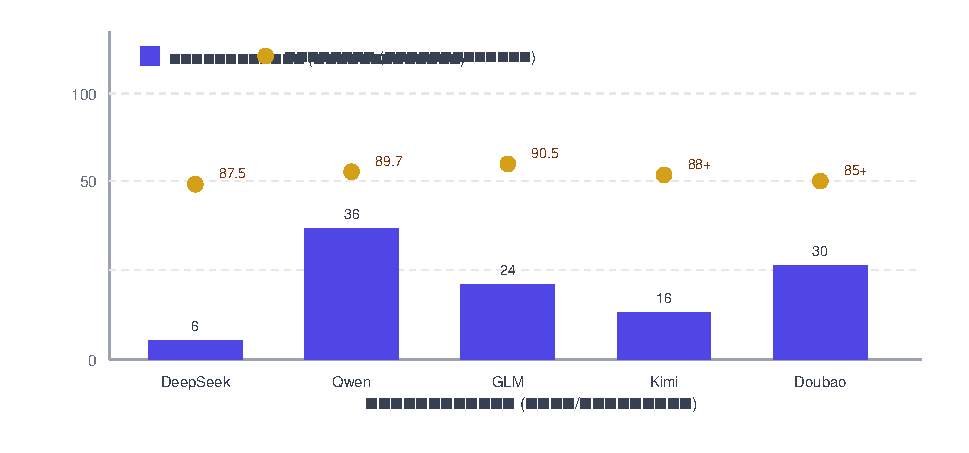
\includegraphics[width=0.92\linewidth]{figures/fig-di-si-shi-er-zhang-1}
\\[2pt]\small ภาพที่ 4: เปรียบเทียบราคากับประสิทธิภาพของโมเดลห้าตัว (ราคายิ่งต่ำยิ่งดี คะแนนยิ่งสูงยิ่งดี)
\end{center}

\booksection{กรอบการตัดสินใจเลือกโมเดล}

รู้จักจุดเด่นของแต่ละโมเดลแล้ว แล้วจะเลือกโมเดลให้โปรเจกต์ของตัวเองอย่างไรดี? ขอแถมวิธี “ตัดสินใจด้วยสี่คำถาม” — ตอบครบสี่ข้อแล้วคุณจะล็อกโมเดลที่เหมาะกับคุณที่สุดได้

โปรเจกต์ของคุณจะใช้ในจีนหรือต่างประเทศ?

ในจีน เลือกโมเดลจีน

|

ต่างประเทศ เลือกโมเดลต่างชาติได้

งานหลักคือเขียนโค้ดหรืออย่างอื่น?

เขียนโค้ด Claude หรือ DeepSeek

|

อื่น ๆ พิจารณาต่อ

ต้องการคอนเท็กซ์ยาวพิเศษ (>500K โทเคน) หรือไม่?

ต้องใช้ Gemini หรือ Kimi

|

ไม่ต้องใช้ พิจารณาต่อ

งบจำกัดไหม?

ละเอียดอ่อน DeepSeek หรือ Qwen-turbo

|

ไม่ละเอียดอ่อน GPT-5.6 หรือ Claude

\begin{center}\small\color{gray}ภาพที่ 5: วิธีตัดสินใจเลือกโมเดลใหญ่ด้วยสี่คำถาม\end{center}

\begin{tcbinfo}{เคล็ดลับ: กลยุทธ์การจับคู่ใช้}
วิธีนี้ไม่ใช่กฎเหล็ก — หลายสถานการณ์ต้องใช้หลายโมเดลร่วมกัน กลยุทธ์จับคู่ที่พบบ่อย: ใช้ DeepSeek หรือ Qwen ทำงานพัฒนาประจำวัน (ต้นทุนต่ำ ภาษาจีนเก่ง) ใช้ Claude ออกแบบสถาปัตยกรรมจุดสำคัญ (reasoning แรง hallucination ต่ำ) ใช้ Gemini ทำการวิเคราะห์มัลติโมดัล (จัดการรูปภาพวิดีโอ) สลับโมเดลตามงาน อย่า “รักโมเดลเดียวใช้ไปตลอด”

\end{tcbinfo}

\booksection{เริ่มต้นเรียก API: ต่อโมเดลใหญ่ตั้งแต่ศูนย์}

บทเรียนเขียนโค้ด AI จำนวนมากสอนแค่วิธีใช้หน้าจอแชท แต่ “การเขียนโค้ด AI” แท้จริง — ที่แอปของคุณเรียกใช้โมเดลใหญ่ — ต้องผ่าน API API (Application Programming Interface) คือโปรโตคอลการสื่อสารระหว่างโปรแกรม ผ่าน API โค้ดของคุณเรียกใช้ความสามารถของโมเดลใหญ่ได้เหมือนเรียกใช้ฟังก์ชันหนึ่งตัว

\booksubsection{Token คืออะไร}

ก่อนจะเข้าใจ API ต้องเข้าใจแนวคิด “Token” ก่อน Token คือหน่วยพื้นฐานของการคิดเงินโมเดลใหญ่ พอเข้าใจง่าย ๆ ว่าเป็น “หน่วยอ่านและหน่วยเขียนของ AI” หนึ่ง Token คร่าว ๆ คือ: ภาษาอังกฤษราว 0.75 คำ (4 ตัวอักษร) ภาษาจีนราว 0.5-1 ตัวอักษร ข้อความจีนยาว 1000 ตัวอักษร กิน Token ราว 1500-2000 Token

Token ไม่ใช่จำนวนคำ ก็ไม่ใช่จำนวนตัวอักษร โมเดลใหญ่ใช้ตัวตัดคำ (Tokenizer) เฉพาะทางแบ่งข้อความออกเป็น Token คำเดียวกันจะนับเป็นกี่ Token ขึ้นอยู่กับแต่ละโมเดล — เช่น คำจีนที่แปลว่า “ปัญญาประดิษฐ์” อาจนับได้ 3 Token ใน GPT แต่ 2 Token ใน DeepSeek API ของโมเดลส่วนใหญ่จะคืนจำนวน Token ที่ใช้จริงกลับมา คุณดูได้จาก API response

\begin{tcbinfo}{ประมาณต้นทุน Token อย่างรวดเร็ว}
ภาษาจีน 1 ล้านตัวอักษร คิดเป็นราว 1.5 ล้าน Token ใช้ DeepSeek V4 Flash ประมวลผล input 1 ล้านตัวอักษร + output 1 ล้านตัวอักษร ต้นทุนราว 0.42 ดอลลาร์สหรัฐ (ราว 3 หยวน); ใช้ Claude Fable 5 ประมวลผลปริมาณเท่ากัน ต้นทุนราว 60 ดอลลาร์สหรัฐ (ราว 434 หยวน) นี่แหละเหตุผลว่าทำไมการเลือกโมเดลจึงกระทบต้นทุนโปรเจกต์ของคุณโดยตรง

\end{tcbinfo}

\booksubsection{การขอ API Key}

ก้าวแรกของการใช้ API โมเดลใหญ่คือขอ API Key — คีย์ยืนยันตัวตนยาว ๆ หนึ่งชุด ผู้ให้บริการแต่ละเจ้ามีแพลตฟอร์ม API ของตัวเอง คุณต้องสมัครบัญชีแล้วสร้าง API Key ด้านล่างคือทางเข้าแพลตฟอร์ม API ของโมเดลหลักพร้อมขั้นตอนการขอ:

\begin{center}
\begin{tabularx}{\linewidth}{|X|X|X|X|}
\hline
\textbf{โมเดล} & \textbf{แพลตฟอร์ม API} & \textbf{ขั้นตอนการขอ} & \textbf{โควตาฟรี} \tabularnewline
\hline
DeepSeek & platform.deepseek.com & สมัคร ยืนยันตัวตน สร้าง API Key & โควตาแถมสำหรับผู้ใช้ใหม่ \tabularnewline
Qwen & bailian.aliyun.com (แพลตฟอร์ม Bailian) & ล็อกอินบัญชี Alibaba Cloud เปิดใช้บริการ สร้าง Key & ผู้ใช้ใหม่ทดลองใช้ฟรี \tabularnewline
GLM จาก Zhipu & open.bigmodel.cn & สมัคร ยืนยันตัวตน สร้าง API Key & โควตาแถมสำหรับผู้ใช้ใหม่ \tabularnewline
Kimi & platform.moonshot.cn & สมัคร ยืนยันตัวตน สร้าง API Key & โควตาฟรีแบบจำกัด \tabularnewline
Doubao & volcengine.com (Volcano Engine) & สมัคร เปิดใช้แพลตฟอร์ม Ark สร้าง API Key & สมัครรับ Token แถมจำนวนมาก \tabularnewline
OpenAI GPT & platform.openai.com & สมัคร ผูกบัตรเครดิต สร้าง API Key & ไม่มีโควตาฟรี (ต้องจ่ายเงิน) \tabularnewline
Anthropic Claude & console.anthropic.com & สมัคร ผูกบัตร สร้าง API Key & ผู้ใหม่ได้โควตาเล็กน้อย \tabularnewline
\hline
\end{tabularx}
\end{center}

\begin{center}\small\color{gray}แพลตฟอร์ม API ของโมเดลหลักและวิธีขอ Key (สิงหาคม 2026)\end{center}

\textbf{คำเตือนความปลอดภัย: API Key = รหัสกระเป๋าเงินของคุณ}\par

API Key เทียบเท่ารหัสกระเป๋าเงินของคุณ — ใครได้ Key ไปก็ใช้โควตาของคุณเรียกโมเดลได้หมด ดังนั้น: อย่าเขียน API Key ลงในโค้ดเด็ดขาด (จัดการด้วย environment variable); อย่า push โค้ดที่มี Key ขึ้น Git repo สาธารณะเด็ดขาด; อย่าแชร์ภาพหน้าจอที่มี Key ลงโซเชียลมีเดียเด็ดขาด ถ้า Key หลุด ให้ลบทิ้งบนแพลตฟอร์มทันทีแล้วสร้างใหม่

\booksubsection{การเรียก API ครั้งแรก}

ได้ API Key แล้ว คุณเรียก API โมเดลใหญ่ได้ด้วยภาษาโปรแกรมใดก็ได้ ด้านล่างใช้ Python สาธิตการเรียกที่ง่ายที่สุด — ส่งข้อความหนึ่งข้อความไปหา DeepSeek แล้วรับคำตอบกลับมา

\begin{lstlisting}[language=Python]
# ติดตั้ง SDK: pip install openai
# DeepSeek ใช้รูปแบบ OpenAI SDK ได้ตรง ๆ
from openai import OpenAI
import os

# 1. สร้าง client (อ่าน API Key จากตัวแปรสภาพแวดล้อม)
client = OpenAI(
    api_key=os.environ.get("DEEPSEEK_API_KEY"),
    base_url="https://api.deepseek.com"
)

# 2. ส่งคำขอ
response = client.chat.completions.create(
    model="deepseek-chat",  # เลือกโมเดล
    messages=[
        {"role": "system", "content": "คุณคือผู้ช่วยเขียนโค้ด Python"},
        {"role": "user", "content": "เขียนฟังก์ชัน quick sort ให้หน่อย"}
    ]
)

# 3. รับคำตอบ
print(response.choices[0].message.content)

# 4. ดูการใช้ Token
print(f"Token เข้า: {response.usage.prompt_tokens}")
print(f"Token ออก: {response.usage.completion_tokens}")
print(f"Token รวม: {response.usage.total_tokens}")
\end{lstlisting}

ตรรกะหลักของโค้ดนี้คือ: สร้าง client (พร้อม API Key และที่อยู่โมเดล) ประกอบลิสต์ข้อความ (system กำหนดบทบาท, user คือ input ของผู้ใช้) ส่ง request รับคำตอบ รูปแบบนี้ใช้ได้กับโมเดลที่รองรับฟอร์แมต OpenAI เกือบทั้งหมด — แค่เปลี่ยน api\_key กับ base\_url ก็สลับโมเดลได้ นี่คือเหตุผลที่โมเดลจีนจำนวนมากเลือกรองรับฟอร์แมต OpenAI SDK: นักพัฒนาแก้แค่สองบรรทัดก็เปลี่ยนโมเดลได้ ต้นทุนการย้ายต่ำมาก

ด้านล่างคือความต่างของโค้ดเมื่อสลับไปใช้โมเดลอื่น — สังเกตว่าแก้แค่สองบรรทัดเท่านั้น:

\begin{lstlisting}[language=Python]
# DeepSeek
client = OpenAI(
    api_key=os.environ.get("DEEPSEEK_API_KEY"),
    base_url="https://api.deepseek.com"
)
# model="deepseek-chat"

# Qwen (แพลตฟอร์ม Bailian)
client = OpenAI(
    api_key=os.environ.get("DASHSCOPE_API_KEY"),
    base_url="https://dashscope.aliyuncs.com/compatible-mode/v1"
)
# model="qwen-plus"

# Zhipu GLM
client = OpenAI(
    api_key=os.environ.get("GLM_API_KEY"),
    base_url="https://open.bigmodel.cn/api/paas/v4"
)
# model="glm-4"

# OpenAI GPT
client = OpenAI(
    api_key=os.environ.get("OPENAI_API_KEY"),
    # base_url ใช้ค่าเริ่มต้นได้เลย
)
# model="gpt-5.6-terra"
\end{lstlisting}

\booksubsection{การจัดการ streaming response}

ในแอปจริง คุณมักไม่อยากรอ AI เขียนจบทุกอย่างแล้วค่อยแสดงทีเดียว — ผู้ใช้จะรอนานเกินไป streaming response ทำให้คุณแสดงทีละคำไปพร้อมกับที่ AI กำลังสร้าง ประสบการณ์ผู้ใช้ดีขึ้นอย่างมหาศาล เหมือนเครื่องพิมพ์ดีด ตัวอักษรเด้งออกมาทีละตัว ความรู้สึกของผู้ใช้ต่างกันสนิท

\begin{lstlisting}[language=Python]
# สตรีม: พิมพ์ทีละตัวอักษร
stream = client.chat.completions.create(
    model="deepseek-chat",
    messages=[
        {"role": "user", "content": "เขียนบทเรียน bubble sort ด้วย Python"}
    ],
    stream=True  # เปิดโหมดสตรีม
)

# รับทีละชิ้นแล้วพิมพ์
for chunk in stream:
    if chunk.choices[0].delta.content is not None:
        print(chunk.choices[0].delta.content, end="", flush=True)
# ผลลัพธ์จะไหลทีละตัวอักษรเหมือนเครื่องพิมพ์ดีด
\end{lstlisting}

\booksection{คู่มือซื้อ Token Plan}

ผู้ให้บริการโมเดลส่วนใหญ่มีสองรูปแบบการคิดเงิน: จ่ายตามการใช้ (Pay-as-you-go) กับแพ็กเกจรายเดือน (Token Plan / Subscription) เข้าใจความต่างของสองแบบนี้แล้วจะช่วยลดต้นทุนการใช้งานของคุณได้มาก

\booksubsection{จ่ายตามการใช้ vs แพ็กเกจรายเดือน}

\begin{center}
\begin{tabularx}{\linewidth}{|X|X|X|}
\hline
\textbf{มุมเปรียบเทียบ} & \textbf{จ่ายตามการใช้ (Pay-as-you-go)} & \textbf{แพ็กเกจรายเดือน (Subscription)} \tabularnewline
\hline
วิธีคิดเงิน & ใช้เท่าไรก็จ่ายเท่านั้น & จ่ายเหมาล่วงหน้า รับโควตามา \tabularnewline
สถานการณ์ที่เหมาะ & ปริมาณใช้ไม่แน่นอน นาน ๆ เรียกที & ปริมาณใช้นิ่ง เรียกใช้บ่อยมาก \tabularnewline
ข้อดีด้านราคา & ราคามาตรฐาน & ถูกกว่าแบบจ่ายตามการใช้ 20\%-50\% \tabularnewline
ความยืดหยุ่น & ใช้ได้ตลอด ไม่ต้องผูกมัด & ต้องจ่ายล่วงหน้า โควตาหมดอายุแล้วอาจเสียเปล่า \tabularnewline
กรณีใช้เกินโควตา & คิดเงินตามการใช้อัตโนมัติ & พอเกินโควตาเปลี่ยนไปคิดตามการใช้ \tabularnewline
แพลตฟอร์มตัวแทน & แพลตฟอร์ม API ทางการของแต่ละโมเดล & OpenAI Plus/Pro, Claude Pro, Cursor Pro \tabularnewline
\hline
\end{tabularx}
\end{center}

\begin{center}\small\color{gray}เปรียบเทียบสองรูปแบบการคิดเงิน\end{center}

สำหรับมือใหม่ แนะนำเริ่มจากแบบจ่ายตามการใช้ — ไม่ต้องจ่ายล่วงหน้า ใช้เท่าไรจ่ายเท่านั้น พอปริมาณการใช้รายเดือนของคุณนิ่งในระดับหนึ่งแล้ว (เช่น เกิน 50 หยวนต่อเดือน) ค่อยพิจารณาเปลี่ยนไปใช้แพ็กเกจรายเดือนเพื่อได้ราคาต่อหน่วยที่ถูกลง

\booksubsection{รวมแพ็กเกจรายเดือนของค่ายหลัก}

\begin{center}
\begin{tabularx}{\linewidth}{|X|X|X|X|}
\hline
\textbf{แพ็กเกจ} & \textbf{ค่ารายเดือน} & \textbf{สิ่งที่ได้รับ} & \textbf{เหมาะกับใคร} \tabularnewline
\hline
ChatGPT Free & ฟรี & แชทข้อความไม่จำกัดด้วย GPT-5.6 Luna & มือใหม่มาลองของ \tabularnewline
ChatGPT Plus & US\$20/เดือน & GPT-5.6 Sol, สร้างรูปภาพ, วิเคราะห์ข้อมูล, เข้าถึงปลั๊กอิน & ผู้ใช้ระดับกลาง \tabularnewline
ChatGPT Pro & US\$200/เดือน & ใช้ทุกโมเดลไม่จำกัด เข้าใช้ฟีเจอร์ใหม่ก่อนใคร & ผู้ใช้หนักระดับมืออาชีพ \tabularnewline
Claude Free & ฟรี & แชท Claude ได้จำกัดจำนวนครั้ง & มือใหม่มาลองของ \tabularnewline
Claude Pro & US\$20/เดือน & ใช้ Claude ไม่จำกัด เข้าถึงโมเดลใหม่ก่อนใคร & นักพัฒนาสายเขียนโค้ด \tabularnewline
Cursor Free & ฟรี & เติมโค้ด AI กับแชทได้จำกัดจำนวนครั้ง & มือใหม่มาลองใช้ \tabularnewline
Cursor Pro & US\$20/เดือน & เติมโค้ด AI ไม่จำกัด, request ระดับสูง 500 ครั้ง/เดือน & นักพัฒนาประจำวัน \tabularnewline
Cursor Business & US\$40/เดือน/คน & ทำงานเป็นทีม, หลังบ้านสำหรับผู้ดูแล, โหมดความเป็นส่วนตัว & ใช้ในทีม \tabularnewline
\hline
\end{tabularx}
\end{center}

\begin{center}\small\color{gray}แพ็กเกจรายเดือนของเครื่องมือ AI ค่ายหลัก (สิงหาคม 2026)\end{center}

แผนรายเดือนของโมเดลจีนต่างออกไปนิดหน่อย DeepSeek เน้นคิดเงินตามการใช้ ไม่มีแพ็กเกจรายเดือน — เติมเงินแล้วหักตามปริมาณที่ใช้จริง Qwen มี resource pack แบบเติมล่วงหน้าบนแพลตฟอร์ม Bailian (ซื้อโควตา Token จำนวนหนึ่งได้ราคาส่วนลด) Doubao บน Volcano Engine ก็มีแผนเติมล่วงหน้าคล้ายกัน สำหรับนักพัฒนาในจีน คอมโบที่คุ้มที่สุดมักเป็น: DeepSeek แบบจ่ายตามการใช้ (พัฒนาประจำวัน) + โควตาฟรีของ Doubao (ลองของกับเทสต์)

\booksubsection{แพลตฟอร์มรวม API}

ถ้าคุณต้องใช้หลายโมเดลพร้อมกัน แพลตฟอร์มรวม API คือทางเลือกที่เบาสมอง แพลตฟอร์มรวมให้ API Key เดียวแบบรวมศูนย์ คุณเรียกโมเดลทั่วโลกได้หลายสิบตัว ไม่ต้องไปสมัครแยกทีละแพลตฟอร์ม

\begin{center}
\begin{tabularx}{\linewidth}{|X|X|X|X|}
\hline
\textbf{แพลตฟอร์ม} & \textbf{จุดเด่น} & \textbf{ข้อดีด้านราคา} & \textbf{สถานการณ์ที่เหมาะ} \tabularnewline
\hline
OpenRouter (openrouter.ai) & แพลตฟอร์มรวมฝั่งต่างประเทศ Key เดียวเรียกโมเดลทั่วโลก & ราคาโปร่งใส เทียบราคาสดได้ & คนที่ต้องสลับใช้หลายโมเดลต่างประเทศแบบยืดหยุ่น \tabularnewline
SiliconFlow (siliconflow.cn) & แพลตฟอร์มรวมฝั่งจีน มี API โมเดลจีนให้เลือกหลายตัว & ถูกกว่าราคาทางการ 20\%-30\% & นักพัฒนาในจีน ที่อยากเทียบราคาหลายโมเดล \tabularnewline
Azure OpenAI (ตัวแทนของ Microsoft) & OpenAI API ผ่านตัวแทน Azure ของ Microsoft & ใช้ Batch API ได้ลดครึ่งราคา & เรียก OpenAI ระดับองค์กร งาน async ปริมาณมาก \tabularnewline
Baidu Qianfan (qianfan.baidubce.com) & แพลตฟอร์ม AI คลาวด์ของ Baidu ให้บริการโมเดลอย่าง Wenxin (ERNIE) & เครดิตฟรีสำหรับผู้ใช้ใหม่ & ผู้ใช้ในระบบนิเวศของ Baidu \tabularnewline
\hline
\end{tabularx}
\end{center}

\begin{center}\small\color{gray}แพลตฟอร์มรวม API หลัก (สิงหาคม 2026)\end{center}

\textbf{เตือนเรื่องกับดัก: อย่าซื้อ “Shared Key”}\par

อย่าซื้อ “API Key แบบใช้ร่วมกัน” จากแพลตฟอร์มอย่าง Taobao หรือ Xianyu—Key พวกนี้มักไม่รู้ที่มาที่ไป อาจถูกระงับบัญชีได้ทุกเมื่อ และยังเสี่ยงข้อมูลรั่วไหลด้วย ให้ขอรับ API Key จากแพลตฟอร์มทางการหรือแพลตฟอร์มรวมที่น่าเชื่อถือเสมอ

\booksubsection{กลยุทธ์ลดต้นทุน}

เลือกโมเดลให้ถูกเป็นแค่ก้าวแรก วิธี “ใช้อย่างคุ้มค่า” ก็สำคัญไม่แพ้กัน นี่คือกลยุทธ์ลดต้นทุนที่ผ่านการใช้จริงพิสูจน์แล้วว่าได้ผล:

\begin{enumerate}
  \item ใช้ cache hit ให้เป็น หลายโมเดลมีฟีเจอร์ "แคช"—เมื่อคำขอของคุณมีเนื้อหาที่เคยประมวลผลมาก่อนหน้า (เช่น system prompt) ส่วนนั้นจะถูกคิดค่าบริการในราคาถูกพิเศษ cache hit ของ DeepSeek มีราคาเพียง 1/60 ของราคาปกติ วาง system prompt ส่วนที่คงที่ไว้ต้นรายการข้อความ จะเพิ่มอัตรา cache hit ได้สูงสุด
  \item จัดชั้นการเรียกใช้—ให้โมเดลราคาถูกจัดการงานง่าย โมเดลแพงจัดการงานซับซ้อน เช่น ใช้ DeepSeek V4 Flash ทำการจัดประเภทข้อความ (เอาต์พุต 2 หยวน/ล้าน Token) และใช้ Claude ทำการออกแบบสถาปัตยกรรม (เอาต์พุต 181 หยวน/ล้าน Token) ในโปรเจกต์หนึ่ง 80\% ของการเรียกใช้ใช้โมเดลราคาถูกได้
  \item จำกัดความยาวเอาต์พุต API คิดค่าบริการตาม Token ฝั่งเอาต์พุต ยิ่งยาวยิ่งแพง ในสถานการณ์ที่ไม่ต้องการข้อความยาว ๆ ให้ตั้งพารามิเตอร์ max\_tokens จำกัดความยาวเอาต์พุต กันไม่ให้ AI "พูดเยอะเปล่า ๆ"
  \item ใช้ Batch API กับงานที่ไม่ต้องเรียลไทม์ ถ้าคุณมีงานจำนวนมากที่ไม่ต้องการคำตอบทันที (เช่น ติดป้ายข้อมูลเป็นชุด สรุปเอกสารเป็นชุด) การใช้ Batch API จะได้ส่วนลด 50\% ทั้ง OpenAI และ Azure มีฟีเจอร์นี้
  \item ติดตามการใช้ Token แพลตฟอร์ม API ส่วนใหญ่มีแดชบอร์ดสถิติการใช้งาน หมั่นดูการกระจายการใช้เป็นระยะ หาการเรียกใช้ที่กิน Token มากที่สุดแล้วปรับแบบตรงจุด การปรับ Prompt เล็ก ๆ น้อยนิด (เช่น เปลี่ยน "อธิบายอย่างละเอียด" เป็น "อธิบายให้อยู่ใน 3 ประโยค") อาจประหยัด Token ได้ถึง 50\%
\end{enumerate}

\begin{center}
\begin{tabularx}{\linewidth}{|X|X|X|X|}
\hline
\textbf{กลยุทธ์} & \textbf{ระดับการประหยัด} & \textbf{ความยากในการทำ} & \textbf{คำอธิบาย} \tabularnewline
\hline
Cache hit & สูงสุด 98\% & ต่ำ & วางเนื้อหาคงที่ไว้ต้นข้อความ \tabularnewline
จัดชั้นการเรียกใช้ & 50\%-80\% & กลาง & งานง่ายใช้โมเดลราคาถูก \tabularnewline
จำกัดความยาวเอาต์พุต & 30\%-60\% & ต่ำ & ตั้งค่าพารามิเตอร์ max\_tokens \tabularnewline
Batch API & 50\% & ต่ำ & งานไม่เรียลไทม์ใช้ batch processing \tabularnewline
ปรับแต่ง Prompt & 20\%-50\% & กลาง & ทำ Prompt ให้กระชับ ลดส่วนซ้ำซ้อน \tabularnewline
\hline
\end{tabularx}
\end{center}

\begin{center}\small\color{gray}กลยุทธ์ลดต้นทุนและผลลัพธ์ (สิงหาคม 2026)\end{center}

\booksection{ลงมือจริง: เชื่อมต่อ API โมเดลใหญ่ในโปรเจกต์}

ปิดบทนี้ด้วยการลงมือจริงแบบครบวงจร—สร้าง “เครื่องสรุปความด้วย AI”: ผู้ใช้ป้อนข้อความยาว ๆ แล้วเรียกใช้ API โมเดลใหญ่สรุปใจความ แบบฝึกหัดนี้จะโชว์กระบวนการเรียกใช้ API ครบทุกขั้น: ตั้งค่าสภาพแวดล้อม เรียกใช้ API จัดการข้อผิดพลาด และควบคุมต้นทุน

\begin{lstlisting}[language=Python]
# ai_summarizer.py - ตัวสรุปข้อความ AI
import os
from openai import OpenAI

# 1. ตั้งค่า (อ่าน API Key จากตัวแปรสภาพแวดล้อม ห้าม hardcode เด็ดขาด)
client = OpenAI(
    api_key=os.environ.get("DEEPSEEK_API_KEY"),
    base_url="https://api.deepseek.com"
)

def summarize(text: str, max_length: int = 200) -> dict:
    """สรุปข้อความ

    Args:
        text: ข้อความต้นฉบับที่ต้องการสรุป
        max_length: ความยาวสรุปสูงสุด (จำนวน Token)

    Returns:
        dict: มีทั้งสรุปและข้อมูลการใช้ Token
    """
    try:
        response = client.chat.completions.create(
            model="deepseek-chat",
            messages=[
                {
                    "role": "system",
                    "content": "คุณคือเครื่องมือสรุปข้อความ"
                               "สรุปข้อความที่ผู้ใช้ให้มาอย่างกระชับ"
                               "สรุปไม่เกิน 3 ประโยค"
                },
                {
                    "role": "user",
                    "content": f"สรุปข้อความต่อไปนี้:\n\n{text}"
                }
            ],
            max_tokens=max_length,  # จำกัดความยาวผลลัพธ์
            temperature=0.3  # อุณหภูมิต่ำ=นิ่งกว่า
        )

        return {
            "success": True,
            "summary": response.choices[0].message.content,
            "input_tokens": response.usage.prompt_tokens,
            "output_tokens": response.usage.completion_tokens,
            "total_tokens": response.usage.total_tokens
        }

    except Exception as e:
        return {
            "success": False,
            "error": str(e)
        }

# 2. ตัวอย่างการใช้
if __name__ == "__main__":
    long_text = """
    (วางข้อความยาว ๆ ตรงนี้...)
    """

    result = summarize(long_text)

    if result["success"]:
        print(f"สรุป: {result['summary']}")
        print(f"ใช้ Token: {result['total_tokens']}")
        # ประมาณต้นทุน: DeepSeek V4 Flash
        cost = result['total_tokens'] * 0.000004  # ราว 0.4 เซี่ยว/พัน Token
        print(f"ต้นทุนโดยประมาณ: {cost:.4f} หยวน")
    else:
        print(f"เกิดข้อผิดพลาด: {result['error']}")
\end{lstlisting}

โค้ดชุดนี้สะท้อนแนวปฏิบัติที่ดีของการเรียกใช้ API หลายข้อ: อ่าน API Key จากตัวแปรสภาพแวดล้อม ไม่เขียนแปะในโค้ดเด็ดขาด; ฟังก์ชันมีเอกสารอธิบายและ type hint ชัดเจน; ตั้งค่า max\_tokens จำกัดความยาวเอาต์พุต; ตั้ง temperature ต่ำ (0.3) เพื่อผลลัพธ์ที่เสถียรขึ้น; จัดการข้อผิดพลาดครบถ้วน; และคืนค่าข้อมูลการใช้ Token เพื่อติดตามต้นทุน ตอนคุณให้ AI เขียนโค้ดชุดนี้ บอกข้อกำหนดพวกนี้ให้มันฟังได้—มันช่วยทำให้ได้ทั้งหมด

บทเรียนสุดท้ายของบทนี้: โมเดลคือ "กระสุน" วิธีการคือ "ยุทธวิธี" เลือกกระสุนดีช่วยให้รบง่ายขึ้น แต่ยุทธวิธีไม่ดี กระสุนเท่าไรก็แพ้ได้ เมื่อรู้จักจุดเด่นของแต่ละโมเดลและวิธีใช้ API แล้ว คุณก็มี "คลังกระสุน" เต็มที่—แต่จะรบยังไงให้ชนะ ต้องพึ่งวิธีคิดที่เรียนมาในบทก่อน ๆ

\begin{tcbpractice}{ลงมือทำ: เรียกใช้ API ครั้งแรกให้ผ่าน}
สมัครแพลตฟอร์มโมเดลจีนสักที่หนึ่ง (แนะนำ DeepSeek หรือ Zhipu ทั้งคู่แจกเครดิตผู้ใช้ใหม่) สร้าง API Key แล้วใส่ไว้ในตัวแปรสภาพแวดล้อมของระบบ (ไม่ใช่ในโค้ด!) จากนั้นรันโค้ด “การเรียกใช้ API ครั้งแรก” ด้านบน วินาทีที่คำตอบของ AI ปรากฏบนหน้าจอ คุณก็ข้ามเส้นแบ่งระหว่าง “ใช้ AI” กับ “สร้างแอป AI” ไปแล้ว

\end{tcbpractice}

\begin{tcbsummary}{สรุปบทนี้}
\begin{itemize}
  \item สามจ่าสากล: GPT-5.6 (สมดุลรอบด้าน), Claude (เพดานสูงสุดด้านเขียนโค้ด + อัตราหลอนเพียง 1\%), Gemini (ราชามัลติโมดัล + บริบท 2 ล้าน Token)
  \item ห้าแชมป์สายจีน: DeepSeek V4 (ราชาคุ้มค่า ระวังประกาศขึ้นราคา), Qwen3.7 (ระดับองค์กร), GLM-5.1 (อันดับ 1 ด้าน SWE ของจีน), Kimi K3 (ข้อความยาวพิเศษ), Doubao (ฟรีสำหรับเริ่มต้น)
  \item วิธีตัดสินใจ 4 คำถาม: ดีพลอยไว้ที่ไหน? เขียนโค้ดหรืองานอื่น? ต้องบริบทยาวพิเศษไหม? งบประมาณอ่อนไหวไหม?
  \item Token คือหน่วยคิดเงิน: ภาษาจีน 1 ตัวอักษร $\approx$ 1.5-2 Token; 1 ล้านตัวอักษร $\approx$ 1.5 ล้าน Token
  \item API Key = รหัสกระเป๋าเงิน: จัดการด้วยตัวแปรสภาพแวดล้อม ห้ามเขียนแปะในโค้ด ห้ามอัปโหลดขึ้น Git
  \item โมเดลจีนส่วนใหญ่ใช้ร่วมกับ OpenAI SDK ได้: เปลี่ยนโมเดลแค่แก้สองบรรทัดคือ api\_key และ base\_url
  \item 5 เทคนิคประหยัดเงิน: cache hit, จัดชั้นการเรียกใช้, จำกัดเอาต์พุต, Batch API, ติดตามการใช้งาน
\end{itemize}

\end{tcbsummary}
